% !TEX TS-program = pdflatex
% !TEX encoding = UTF-8 Unicode

% This is a simple template for a LaTeX document using the "article" class.
% See "book", "report", "letter" for other types of document.

\documentclass[11pt]{article} % use larger type; default would be 10pt

\usepackage[utf8]{inputenc} % set input encoding (not needed with XeLaTeX)
\usepackage{graphicx}
\graphicspath{ {images/} }
%%% Examples of Article customizations
% These packages are optional, depending whether you want the features they provide.
% See the LaTeX Companion or other references for full information.

%%% PAGE DIMENSIONS
\usepackage{geometry} % to change the page dimensions
\geometry{a4paper} % or letterpaper (US) or a5paper or....
% \geometry{margin=2in} % for example, change the margins to 2 inches all round
% \geometry{landscape} % set up the page for landscape
%   read geometry.pdf for detailed page layout information

\usepackage{graphicx} % support the \includegraphics command and options

% \usepackage[parfill]{parskip} % Activate to begin paragraphs with an empty line rather than an indent

%%% PACKAGES
\usepackage{booktabs} % for much better looking tables
\usepackage{array} % for better arrays (eg matrices) in maths
\usepackage{paralist} % very flexible & customisable lists (eg. enumerate/itemize, etc.)
\usepackage{verbatim} % adds environment for commenting out blocks of text & for better verbatim
\usepackage{subfig} % make it possible to include more than one captioned figure/table in a single float
% These packages are all incorporated in the memoir class to one degree or another...

%%% HEADERS & FOOTERS
\usepackage{fancyhdr} % This should be set AFTER setting up the page geometry
\pagestyle{fancy} % options: empty , plain , fancy
\renewcommand{\headrulewidth}{0pt} % customise the layout...
\lhead{}\chead{}\rhead{}
\lfoot{}\cfoot{\thepage}\rfoot{}

%%% SECTION TITLE APPEARANCE
\usepackage{sectsty}
\allsectionsfont{\sffamily\mdseries\upshape} % (See the fntguide.pdf for font help)
% (This matches ConTeXt defaults)

%%% ToC (table of contents) APPEARANCE
\usepackage[nottoc,notlof,notlot]{tocbibind} % Put the bibliography in the ToC
\usepackage[titles,subfigure]{tocloft} % Alter the style of the Table of Contents
\renewcommand{\cftsecfont}{\rmfamily\mdseries\upshape}
\renewcommand{\cftsecpagefont}{\rmfamily\mdseries\upshape} % No bold!

%%% END Article customizations

%%% The "real" document content comes below...

\title{Face Tracking for Optimized Bitrate Control in Low Delay Video Encoding}
\author{Chethan Ningaraju}
%\date{} % Activate to display a given date or no date (if empty),
         % otherwise the current date is printed 

\begin{document}
\maketitle

\section{Introduction}
  \subsection{Low Delay Bitrate Control}
	In recent years there is increasing demand for high quality video conferencing solutions. To address this growing need there has been constant improvement in  low delay video coding techniques. The need for extremely low end to end delay in video telephony puts additional contraints on video coding which results in compromise of video quality.

	The bitrate control module is responsible for controlling the bit-consumption of the encoder to guarantee smooth playback. Bitrate control module is not codec specific and operates independent of any chosen codec. The main purpose of the bitrate control module is to ensure efficient playback of the encoded video. Figure 1 shows the functionality the bitrate control module. It achieves this by controlling the quantization parameter using during the encoding. The decision of quantization parameter is done considering the input bitrate, framerate, input complexity (spatial and temporal activity), acceptable input delay (a measure of VBV buffer size). The module also takes the feedback from the encoder regularly to make better decision.  During the low delay video encoding, tools like bi-directional  	prediction are disabled.

\begin{figure}[h]
    \centering
    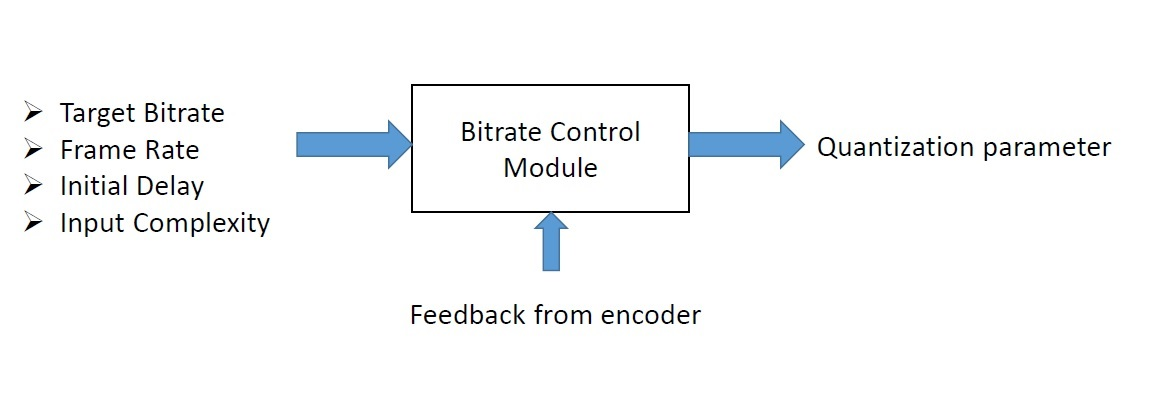
\includegraphics[scale=0.5]{RC_block}
    \caption{Bitrate Control Module Functionality}
    \label{fig:Bitrate Control Module Functionality}
\end{figure} 

  \subsection{ROI based coding}
	In conventional video coding, all regions of the frame is considered equally important. It is assumed all regions contribute equally for perceptual quality. Some video codecs use the fact that high frequency components are less important to human visual system and do you preferential coding based on spatial frequency. However, such prefential coding does not take into account the contents the frame to be encoded. 

Region of interest based coding is not a common practice in video coding because it is very hard to automatically detect important regions that contribute the most to perceptual quality. However, region of interest in video conferencing content is going to be face region predominantly. Due to recent improvements in face detection algorithms it is possible to detect face with good accuracy. This work aims to study possible ways of improving preceptual quality of the video by detecting face regions and coding it with higher quality than rest of the frame.

\section{Operating Conditions}     
This work uses Citrix h264 video codec for the study. The encoder is configured in low delay mode sutiable for video conferencing. The encoder is configured to use IPPP mode with intra/key frames encoded only at the beginning of the sequence. Due to low delay there is no provision to re-encode the frame in case of buffer overflow. The frames are skipped entirely in case of buffer overflow to guarantee smoother playback by maintaning the delay constant. 

The quantization paramter is adapted at every maco-block level to meet the overall bitrate 


\end{document}
